\renewcommand*{\arraystretch}{1.1}

\noindent\begin{tabularx}{17cm}{|>{\small \sf}c|X|}
	\hline
	query    & Interactive / complex / 13 \\ \hline
%
	title       & Single shortest path \\ \hline
%
    pattern     & \hfill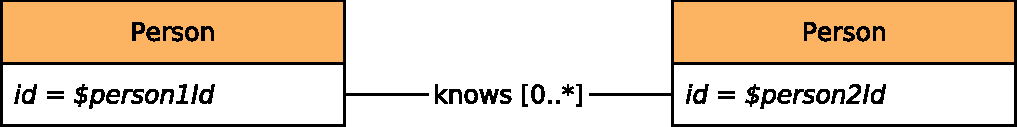
\includegraphics[scale=\patternscale,margin=0cm .2cm]{patterns/interactive-complex-read-13}\hfill\vadjust{} \\ \hline
%
	desc. & Given two Persons, find the shortest path between these two Persons in
the subgraph induced by the Knows relationships.

Return the length of this path:

\begin{itemize}
\tightlist
\item
  -1 : no path found
\item
  0: start person = end person
\item
  \textgreater{} 0: regular case
\end{itemize}
 \\ \hline
%
	
%
	params  &
	\vspace{1.1ex}{\begin{tabularx}{14.66cm}{|c|M|m{2cm}|Y|} \hline
	\cellcolor{parameter} \color{white} \footnotesize $\mathsf{1}$ & \varname{person1.id} & \cellcolor{gray!20} \vartype{ID} &  \\ \hline
	\cellcolor{parameter} \color{white} \footnotesize $\mathsf{2}$ & \varname{person2.id} & \cellcolor{gray!20} \vartype{ID} &  \\ \hline
	\end{tabularx}}\vspace{1.1ex} \\ \hline
%
	
	result      &
	\vspace{1.1ex}{\begin{tabularx}{14.66cm}{|c|M|m{2cm}|c|Y|} \hline
	\cellcolor{result} \color{white} \footnotesize $\mathsf{1}$ & \varname{length} & \cellcolor{gray!20} \vartype{32-bit Integer} &
	    \texttt{C} &
	     \\ \hline
	\end{tabularx}}\vspace{1.1ex} \\ \hline
	
%
	%
	%
	CPs &
	\multicolumn{1}{>{\raggedright}l|}{
	  \chokepoint{3.3}, 
	  \chokepoint{7.2}, 
	  \chokepoint{7.3}
	  } \\ \hline
	%
    relevance &
      \small This query looks for a variable length path, starting at a given Person and finishing at an another given Person.
Proper cardinality estimation and search space prunning, will be crucial. This query also allows for possible parallel
implementations.
 \\ \hline%
\end{tabularx}
\vspace{2ex}